\documentclass[border=8pt]{standalone}
\usepackage{tikz}
\usepackage{amsmath,amssymb}
\usetikzlibrary{arrows.meta, positioning, calc, fit, backgrounds, decorations.pathreplacing}

\definecolor{accent}{HTML}{1B4F72}
\definecolor{accentdeep}{HTML}{0E2F44}
\definecolor{accentmid}{HTML}{2E86C1}
\definecolor{accentlight}{HTML}{EBF5FB}
\definecolor{gold}{HTML}{D4AC0D}
\definecolor{goldlight}{HTML}{FFF8DC}
\definecolor{bordersoft}{HTML}{BDC3C7}
\definecolor{frozenblock}{HTML}{E8E8E8}
\definecolor{textmuted}{HTML}{888888}
\definecolor{redalert}{HTML}{C0392B}
\definecolor{redlight}{HTML}{FDEDEC}
\definecolor{greenok}{HTML}{27AE60}
\definecolor{greenlight}{HTML}{EAFAF1}

\begin{document}
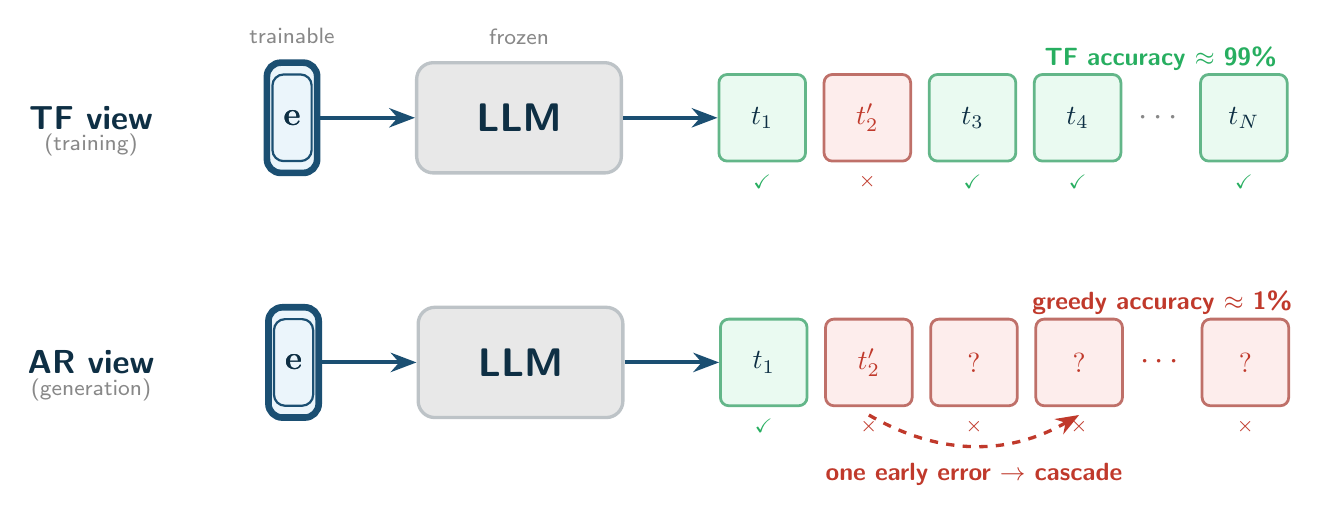
\begin{tikzpicture}[
    >=Stealth,
    font=\sffamily,
    every node/.style={inner sep=0pt},
    embbox/.style={
        draw=accent, line width=2.4pt, rounded corners=5pt,
        fill=accentlight, minimum height=14mm,
        font=\sffamily\bfseries\large, text=accentdeep, align=center,
        inner sep=6pt
    },
    llmbox/.style={
        draw=bordersoft, line width=1.2pt, rounded corners=6pt,
        fill=frozenblock, minimum height=14mm, minimum width=26mm,
        font=\sffamily\bfseries\Large, text=accentdeep, align=center,
        inner sep=6pt
    },
    tok/.style={
        draw=bordersoft, line width=1pt, rounded corners=3pt,
        minimum width=11mm, minimum height=11mm,
        font=\sffamily\normalsize, text=accentdeep, align=center,
        inner sep=2pt
    },
    tokok/.style={tok, fill=greenlight, draw=greenok!60!bordersoft},
    tokerr/.style={tok, fill=redlight, draw=redalert!60!bordersoft,
                   font=\sffamily\normalsize\bfseries, text=redalert},
    arrstyle/.style={->, line width=1.4pt, accent},
    mlabel/.style={font=\sffamily\footnotesize, text=textmuted},
    alabel/.style={font=\sffamily\footnotesize, text=accent},
]

% ============ ROW 1: Teacher-forced (TF) accuracy ============
\node[font=\sffamily\bfseries\large, text=accentdeep] (label1) {TF view};
\node[mlabel, below=0.5mm of label1] (sub1) {(training)};

% Embedding
\node[embbox, right=14mm of label1] (emb1) {$\mathbf{e}$};
\node[draw=accent, line width=0.8pt, rounded corners=4pt,
      minimum height=11mm, inner sep=4pt,
      font=\sffamily\bfseries\large, text=accentdeep] at (emb1.center) {$\mathbf{e}$};
\node[mlabel, above=2mm of emb1] {trainable};

% LLM
\node[llmbox, right=12mm of emb1] (llm1) {LLM};
\node[mlabel, above=2mm of llm1] {frozen};

% Tokens — almost all OK under teacher forcing, but t2 is wrong
\def\tokstart{3.2}
\node[tokok, right=12mm of llm1] (t1a) {$t_1$};
\node[tokerr, right=2mm of t1a] (t2a) {$t_2'$};
\node[tokok, right=2mm of t2a] (t3a) {$t_3$};
\node[tokok, right=2mm of t3a] (t4a) {$t_4$};
\node[font=\sffamily\large, text=textmuted, right=2mm of t4a] (dots1) {$\cdots$};
\node[tokok, right=2mm of dots1] (tna) {$t_N$};

% Arrows
\draw[arrstyle] (emb1.east) -- (llm1.west);
\draw[arrstyle] (llm1.east) -- (t1a.west);

% TF accuracy label
\node[font=\sffamily\small\bfseries, text=greenok, above=5mm of dots1] (tflabel) {TF accuracy $\approx$ 99\%};

% Check / cross marks
\foreach \tok in {t1a, t3a, t4a, tna} {
    \node[font=\sffamily\scriptsize, text=greenok, below=1.5mm of \tok] {\checkmark};
}
\node[font=\sffamily\scriptsize, text=redalert, below=1.5mm of t2a] {$\times$};

% ============ ROW 2: Autoregressive generation ============
\node[font=\sffamily\bfseries\large, text=accentdeep, below=28mm of label1] (label2) {AR view};
\node[mlabel, below=0.5mm of label2] (sub2) {(generation)};

% Embedding
\node[embbox, right=14mm of label2] (emb2) {$\mathbf{e}$};
\node[draw=accent, line width=0.8pt, rounded corners=4pt,
      minimum height=11mm, inner sep=4pt,
      font=\sffamily\bfseries\large, text=accentdeep] at (emb2.center) {$\mathbf{e}$};

% LLM
\node[llmbox, right=12mm of emb2] (llm2) {LLM};

% Tokens — early error cascades
\node[tokok, right=12mm of llm2] (t1b) {$t_1$};
\node[tokerr, right=2mm of t1b] (t2b) {$t_2'$};
\node[tokerr, right=2mm of t2b] (t3b) {$?$};
\node[tokerr, right=2mm of t3b] (t4b) {$?$};
\node[font=\sffamily\large, text=redalert, right=2mm of t4b] (dots2) {$\cdots$};
\node[tokerr, right=2mm of dots2] (tnb) {$?$};

% Arrows
\draw[arrstyle] (emb2.east) -- (llm2.west);
\draw[arrstyle] (llm2.east) -- (t1b.west);

% Error cascade annotation
\draw[->, line width=1.2pt, redalert, dashed]
    ([yshift=-1mm]t2b.south) to[out=-30, in=-150] ([yshift=-1mm]t4b.south);
\node[font=\sffamily\small\bfseries, text=redalert, below=7mm of t3b] (casclabel) {one early error $\rightarrow$ cascade};

% Greedy accuracy label
\node[font=\sffamily\small\bfseries, text=redalert, above=5mm of dots2] (arlabel) {greedy accuracy $\approx$ 1\%};

% Check / cross marks
\node[font=\sffamily\scriptsize, text=greenok, below=1.5mm of t1b] {\checkmark};
\foreach \tok in {t2b, t3b, t4b, tnb} {
    \node[font=\sffamily\scriptsize, text=redalert, below=1.5mm of \tok] {$\times$};
}

\end{tikzpicture}
\end{document}
